\uuid{TsmC}
\exo7id{7165}
\titre{exo7 7165}
\auteur{megy}
\organisation{exo7}
\datecreate{2017-06-11}
\isIndication{true}
\isCorrection{true}
\chapitre{Géométrie affine euclidienne}
\sousChapitre{Géométrie affine euclidienne du plan}
\module{Géométrie}
\niveau{L2}
\difficulte{}

\contenu{
\texte{
Soit $ABC$ un triangle équilatéral direct, et $P$ un point n'appartenant pas aux droites $(AB)$, $(BC)$ et $CA)$. La parallèle à $(BC)$ (resp. à $(CA)$ et $(AB)$) passant par $P$ coupe $(AB)$ (resp. $(BC)$ et $(CA)$) en $U$ (resp. $V$, $W$).

\begin{center}
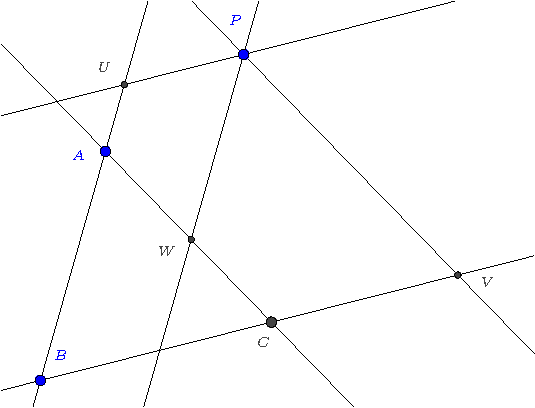
\includegraphics{../images/pdf/TsmC-1.pdf}
\end{center}
}
\begin{enumerate}
    \item \question{Montrer que $AUPW$ et $PCVW$ sont inscriptibles.}
    \item \question{Dresser une liste d'égalités d'angles (de droites) que l'on peut  déduire.}
    \item \question{Faire une (grande) figure dans le cas où $P$ est sur le cercle circonscrit à $ABC$.}
    \item \question{Montrer que les points $U$, $V$ et $W$ sont alignés ssi $ABCP$ est inscriptible.}
\reponse{
Il suffit de montrer que $(AU,AW)=(PU,PW)$. 
\begin{center}
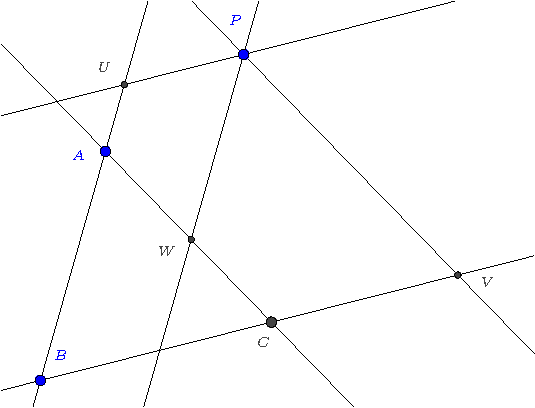
\includegraphics{../images/pdf/TsmC-1.pdf}
\end{center}
Or, on a :
\begin{align*}
(AU,AW)
&= (AB,AC) \text{ (mêmes droites)}\\
&= \pi/3 \text{ (car équilatéral direct)}
\end{align*}
et
\begin{align*}
(PU,PW)
&= (BC,BA) \text{ (droites parallèles donc mêmes angles)}\\
&= \pi/3\text{ (car équilatéral direct)}.
\end{align*}
Donc $(AU,AW)=(PU,PW)$ et donc $APUW$ est inscriptible.

On procède de même pour l'autre quadrilatère.
Pour chaque quadrilatère inscriptible, on peut en déduire  six égalités d'angles inscrits, car il y a $6=\binom{2}{4}$ façons de choisir une corde. Si $APUW$ est inscriptible, on a donc les égalités d'angles de droites:
\[(UA,UP)=(WA,WP),\quad (AU,AW)=(PU,PW),\]
et surtout:
\[ (WA,WU)=(PA,PU)\quad (AU,AP)=(WU,WP),\]
\[ (UP,UW)=(AP,AW),\quad (PW,PA)=(UW,UA).\]
Les plus intéressantes (et utiles pour la suite) sont les quatre dernières.

On procède de même pour l'autre quadrilatère.
Il suffit de montrer que $ABCP$ est inscriptible si et seulement si $(WU,WP)=(WV,WP)$. 
Cette dernière assertion dit en effet que les droites $(WU)$ et $(WV)$ forment le même angle avec $WP$ donc sont parallèles, et donc égales car elles ont le point $W$ en commun.

\begin{center}
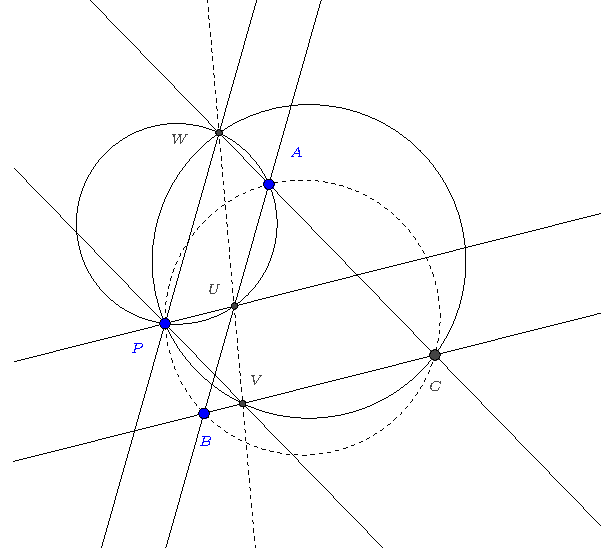
\includegraphics{../images/pdf/TsmC-2.pdf}
\end{center}
On a :
\begin{align*}
(WU,WP)
&= (AU,AP) \text{ (car $AUWP$ est inscriptible)}\\
&= (AB,AP) \text{ (mêmes droites car $U\in (AB)$ )}\\
&= (CB,CP) \text{ \underline{ssi $ABPC$ est inscriptible}}
\end{align*}
et d'autre part, on a 
\begin{align*}
(CB,CP)
&= (CV,CP) \text{ (mêmes droites car $V\in (BC)$ )}\\
&= (WV,WP) \text{ (car $PWCV$ est inscriptible)}
\end{align*}
}
\indication{Dans la dernière question, faire apparaître le point $P$ dans la condition d'alignement à l'aide de la relation de Chasles, par exemple.}
\end{enumerate}
}
